\chapter{Background}\label{chap:background}

This chapter describes various concepts relevant to the rest of this thesis,
starting with an introduction to the system this thesis makes its contributions
to---Soup. Afterwards the Rust programming language is outlined, together with a
look at the \code{bincode} serialization library, which is used for both
snapshotting and persistent base tables. Following that, a few profiling
concepts are described, used to reason about performance issues throughout the
thesis. Finally, the two storage engines embedded in separate implementation
iterations of persistent base tables are studied.

% TODO: this sucks

\newpage

\section{Soup}

Soup~\cite{xylem} is an on-going research project at the Parallel and Distributed Operating
Systems\furl{https://pdos.csail.mit.edu/} group at MIT CSAIL.\@ The current Soup
prototype is written in the Rust programming language and made available as
open-source code on GitHub\furl{https://github.com/mit-pdos/distributary/}.

This section introduces Soup's core concepts.

\subsection{Data-flow}
\todo{figure that compares a traditional query graph to soup's data-flow}

Applications using Soup define base table schemas and a set of queries ahead of
time. Whereas the former is common in traditional relational database management
systems, the latter is not, and is the primary source of Soup's read performance
improvements. A relational database computes the result of queries on-the-fly,
by building a query-graph, which it then executes. This requires potentially
costly computations to be performed multiple times for separate queries, while
throwing away intermediary results that could be re-used. Soup instead builds a
\textit{data-flow} graph from its pre-defined queries, propagating each update
through it at write-time. Computations can then be incrementally maintained on
each write, reducing the work needed by a read-operation to something more
similar to a simple key-value read in a caching system.

\begin{listing}[H]
  \begin{minted}[frame=lines]{sql}
CREATE TABLE Car (id int, brand varchar(255), PRIMARY KEY(id));
QUERY CountCars: SELECT COUNT(*) FROM Car WHERE brand = ?;
  \end{minted}

  \caption{An example base table with a corresponding
  query.}\label{lst:example-schema}
\end{listing}

Implemented naively, incrementally maintaining a data-flow graph for each query
would have disastrous storage consequences. Each query would need a separate
graph, duplicating data across a range of nodes. Instead, Soup builds a single
data-flow graph from all of its queries, recognizing common sub-expressions
where possible~\cite{common-expression}. That still leaves the issue of what
state to incrementally maintain. With queries consisting of a potentially large
amount of nodes, materializing data at each step would lead to significant
overlap between nodes. Instead, Soup only materializes and incrementally
maintains state at nodes it considers \textit{stateful}, with other nodes
referring upwards in the graph to its closest materialized ancestor node.

The state at these materialized nodes is also kept \textit{partial} whenever
possible. Instead of storing the results for all queries---like a materialized
view does---Soup only retains state for records in the application's working
set, evicting rarely used data. Queries for missing keys result in ancestor
queries---\textit{replays}---to nodes further up the graph. Similar to cache
misses in other systems these eventually propagate all the way up to the base
nodes, where a full copy of the state is always maintained.

\subsubsection{Migrations}

Schema migrations are inevitable in long-running applications: business
requirements change, projects are refactored, and new features are added.
Performing migrations in traditional database systems, without downtime, is on
the other hand far from trivial~\cite{stripe, gh-ost}. While Soup requires both
the schema and all queries to be defined ahead of time, it handles changes in
both seamlessly.

Added queries extend the existing data-flow with additional nodes, while
re-using as much as possible of the existing graph. New partially materialized
nodes can start serving requests right away, by fetching data from ancestor
nodes if necessary. This is not the case with fully materialized nodes, which
require a full representation of their state at all times. To bring these nodes
online, Soup incurs a full replay of the state needed, potentially delaying new
requests until all replays have completed. Review of the migrations performed
during the lifetime of the HotCRP conference review
program~\cite{hotcrp}---which uses MySQL---showed that these delays were rare,
with Soup being able to transition 95\% of schema changes without downtime.

\todo{figure of a changing data-flow graph}

Changes to the base table schema happen in-place, and Soup's base nodes retain a
full history of columns for each table. This ensures that both existing and new
requests can be served alongside each other, allowing the data-flow graph to
transition without downtime.

\subsubsection{Domains}

Soup's data-flow graph is partitioned into \textit{domains}, each containing a
series of nodes. Updates are processed at separate domains asynchronously, in
different computational units---threads, or other machines altogether for
distributed Soup. Within a single domain, packets are processed synchronously,
one at a time, removing the need for locking within domains. Packet processing
at domains include both regular updates and other types of packets, such as
replay requests.

\todo{figure that shows different domains}

Domains are separated by egress and ingress nodes, responsible for maintaining
communication across domain boundaries using a buffered channel. When Soup is
run in a distributed fashion, communication between separate domains happen
over TCP sockets, between the egress and ingress nodes.

\subsubsection{Sharding}

Distributing domains across computational units lets Soup divide its processing
load between a cluster of machines. This is only an improvement if the load is
uniformly spread across all domains. When that is not the case, and a majority
of the data is skewed towards a single domain, Soup is left to processing most
of the requests in a single computational unit. This is where sharding comes in.
By splitting the atom that is a single domain into multiple shards, both the
computational load and the data stored at that domain can be spread between
multiple computational units.

\todo{show a figure with a sharder?}

Balancing the data across a cluster is essential in scaling Soup to larger
datasets. Without sharding, Soup's capabilities would be capped at the memory
size of the largest machine in the cluster. Soup shards data by
hash-partitioning keys statically. This is unfortunate for workloads skewed
towards a small key subset, where only a few domains might end up serving most
of the requests received. Dynamic sharding would evenly re-balance the workload
across the shards, and is a future implementation goal for Soup.

When necessary, a \textit{sharder} node is inserted between domains, translating
between sharding schemes in separate domains. This allows nodes further down in
the graph to remain partial, at the cost of having to replay state across
domains.


\subsubsection{Eviction}\label{sec:eviction}

To ensure that partial state does in fact remain partial over time, Soup evicts
data when necessary. Currently this happens when Soup's memory-limit goes beyond
an application-defined limit. This triggers an eviction notice sent to the
largest domain---measured in state-size---which then takes care of propagating
this eviction notice downstream in the graph to any nodes that might depend on
the evicted state.

\todo{might not be necessary, but could have an eviction figure here}

The keys to evict at a specific node are picked randomly. In the future, this
could be improved through more sophisticated eviction strategies, such as only
evicting the least-recently used records.

\subsection{Operators}

Soup's data-flow graph consists of relational operators, where each operator
emits either the \code{Positive} or the \code{Negative} records required for
downstream nodes to maintain their state accordingly.

\subsubsection{Base nodes}

Every packet that reaches Soup is first injected into an appropriate base node,
similar to a table in a relational database. This is where external API requests
are translated into a language the rest of the data-flow graph understands.
While clients might issue \eg deletion requests by \textit{key}, the base nodes
translate the request into a \code{Negative} record for the entire row, which
the rest of the data-flow graph can use to invalidate removed state. Update
requests are likewise first translated into a \code{Negative} record, followed
by a \code{Positive} record containing the new row.

Whereas other stateful nodes can keep their state \textit{partial}, choosing
which records to maintain and which to discard, base nodes always remain fully
materialized at all times.

\subsubsection{Stateless operators}

Stateless operators process updates with no regard for prior events, without
maintaining any state at all. The operators that fall within this category are
\textit{pure functions}, such as the \textit{projection} and \textit{filter}
operators. The former pick out one or more fields from each incoming row, while
the latter determines if a row should be forwarded through the data-flow graph
or not.

While Soup is free to insert operators into its data-flow graph as it sees fit,
both projections and filters can often be mapped directly to a part of an SQL
query. \code{SELECT name \dots} would result in the projection shown in
figure~\ref{fig:project}, while a \code{WHERE}-clause on the form of \code{WHERE
age < 10} would produce a filter operator emitting only records where \code{age
< 10} is true.

\begin{figure}[H]
  \centering
  \includesvg[width=0.3\textwidth]{project}
  \caption{A projection operator responsible for picking out the \code{name}
  column of incoming records.}\label{fig:project}
\end{figure}

\subsubsection{Stateful operators}

Whereas stateless operators resemble their counter-parts in relational
databases~\cite{codd}, Soup's stateful operators compute results incrementally
by maintaining internal state between updates. This saves Soup from re-doing
potentially expensive computations, by instead mutating the previous result when
a new record arrives. The \textit{count} operator---produced by a SQL
\code{COUNT}-clause---is an example of a stateful operator, where
\code{Positive} and \code{Negative} records incur an addition or subtraction of
the current count, respectively. Another example is the \textit{top-k} operator,
produced by \eg an \code{ORDER BY}-clause coupled with a \code{LIMIT} to
determine the $ k $ most significant or insignificant elements.

\begin{figure}[H]
  \centering
  \includesvg[width=0.3\textwidth]{max}
  \caption{\
    The \textit{max} operator emits both a negative and a positive record when
    its state changes: the former to signal that its previous state should be
    invalidated, the latter to inform downstream nodes of the new result.
  }
\end{figure}

\subsubsection{Joins}

Finally, Soup supports joining together multiple paths of the data-flow graph.
This is made possible using \textit{ancestor queries}. Whenever a record arrives
at a join operator, it queries its other ancestors for the records required to
produce a single, unified update. To make sure that this is completed in an
efficient manner, join operators force their ancestors to retain indices on the
fields that they need to be queried for.

\begin{figure}[H]
  \centering
  \includesvg[width=0.7\textwidth]{join}
  \caption{\
    An ancestor query is performed to the right side of the join to produce a
    unified record for the update received from the left.
  }
\end{figure}

\subsection{Eventual consistency}

Databases are often considered the source of truth for applications, and
anomalies here could have disastrous consequences. Whereas fatal failures are
easy to recognize, unexpected behavior at the data layer could be the exact
opposite. This is a convincing argument for strong consistency, where the result
of all operations can be reasoned about from the ordering and type of operation
performed.

Regardless, companies scaling web applications to large amounts of users often
opt for systems with lesser consistency guarantees~\cite{dynamo, pnuts, werner}.
While the performance of strongly consistent systems have taken a turn for the
better with the introduction of horizontally scalable systems with clearly defined
consistency guarantees~\cite{spanner, cockroach}, the race is still far from
even when compared to systems with lesser consistency guarantees. At the same
time, the question of whether strong consistency is actually a requirement for
most applications remain. Analysis of live requests at
Facebook~\cite{existential} showed the opposite: only 0.0004\% of reads would
have returned different results in a strongly consistent system with total
ordering. These cases could then be handled explicitly, avoiding the need to
penalize the performance of an entire system for a fraction of the requests.

Soup targets applications where eventual consistency is sufficient, and would
not be able to provide the performance it does without it. Eventual consistency
avoids the need for explicit synchronization on every update, while allowing
Soup to scale in a distributed fashion without a total ordering of writes.
Clients receive write acknowledgments for writes when updates have been safely
persisted to durable storage, after which they are propagated through Soup's data-flow
graph asynchronously.

Reads access double-buffered hash tables directly~\cite{evmap}, without the need
for locks. Writes update one of the buffers and expose updated content to the
readers with an atomic swap.

\subsection{Architecture}\label{sec:soup-architecture}

\todo{figure}

\subsubsection{Controller}

At the heart of Soup lies a replicated controller, with a leader elected
using ZooKeeper~\cite{zookeeper}. The controller is the first point of contact
for Soup's external APIs, and is responsible for managing meta state, such as
schemas and queries.

\subsubsection{Souplets}

Processing of updates happen within the Souplets---Soup's worker nodes. Each
Souplet includes a pool of threads which together go through the incoming
packets for its domains. While maximum one thread can process updates for a
domain at once, multiple domains can process updates in parallel. Earlier
versions of Soup ran domains in separate threads altogether, resulting in a
core-constrained system when the number of domains went far beyond the host's
CPU core count.

Communication between the Souplets and the controller happens over TCP, at the
coordination layer.

\subsubsection{Readers}

Soup's reader nodes make use of double-buffered hash tables to make it possible
to read and write to a single data structure at the same time. To prevent high
throughput write processing from slowing down reads, read requests are processed
by separate threads---readers.

\subsection{Interacting with Soup}

Applications using Soup define a base table schema and a set of corresponding
queries. The query syntax resembles that of prepared statements in relational
databases, where placeholders are replaced with values when the query is used in
a read operation. Both the schema and the queries can be modified and extended
later on, through Soup's external API.\@

\begin{listing}[H]
  \begin{minted}[frame=lines]{sql}
/* Base table schemas: */
CREATE TABLE Article (aid int, title varchar(255),
                     url text, PRIMARY KEY(aid));
CREATE TABLE Vote (aid int, uid int);

/* Intermediate view (not exposed through the client): */
VoteCount: SELECT Vote.aid, COUNT(uid) AS votes
            FROM Vote GROUP BY Vote.aid;

/* Read query: */
QUERY ArticleWithVoteCount:
            SELECT Article.aid, title, url, VoteCount.votes AS votes
            FROM Article, VoteCount
            WHERE Article.aid = VoteCount.aid AND Article.aid = ?;
  \end{minted}
  \caption{Soup schema with two base tables and an external query.}\label{lst:soup-schema}
\end{listing}

Writing to and reading from Soup is done through mutators and getters. Both are
built by going through the controller, after which writes can go directly to the
domain and reads can access readers directly.

\begin{listing}[H]
  \begin{minted}[frame=lines]{rust}
// Build mutators and getter.
let mut article = blender.get_mutator("Article").unwrap();
let mut vote = blender.get_mutator("Vote").unwrap();
let mut awvc = blender.get_getter("ArticleWithVoteCount").unwrap();

// Insert a new article:
let aid = 1;
let title = "new article";
let url = "https://ntnu.edu";
article
  .put(vec![aid.into(), title.into(), url.into()])
  .unwrap();

// Vote for the article:
let uid = 123;
vote
  .put(vec![aid.into(), uid.into()])
  .unwrap();

// Read the vote count:
println!("{}", awvc.lookup(&[aid.into()], true));
  \end{minted}

  \caption{Soup example usage, where an article and a vote is inserted,
  followed by a read of the vote count.}\label{lst:soup-api}
\end{listing}

\subsection{MySQL Protocol Translation}\label{sec:mysql-shim}

Soup supports a decent subset of SQL in its query definitions. Regardless, using
Soup in an application requires significant changes: all queries have to be
defined ahead of time, and interactions with Soup have to go through Soup's
external API.\@ Soup's MySQL shim~\cite{soup-mysql} makes this easier by letting
applications communicate with Soup using the MySQL binary protocol.

The MySQL shim acts as a separate service, which clients interact with over
TCP.\@ Received queries extend the Soup data-flow graph if needed, before they
are forwarded to an appropriate Soup worker for execution.

% TODO: maybe write a little more

\section{SQLite}\label{sec:sqlite}
SQLite~\cite{sqlite} is by far the most widely deployed database ever written.
Used in everything from smart phones to cars, with an estimated user count in
the magnitude of multiple billion users, SQLite is everywhere\footnote{Who
uses SQLite? \url{https://www.sqlite.org/mostdeployed.html}}. SQlite is an
embedded database, and requires no extra processes, or even threads, to run.

In a world of unreliable software, SQLite is stable as a rock. It has 100\%
branch test coverage, with a test suite containing millions of different test
cases. SQLite is, and always has been, available in the public domain. As the
name implies, SQLite provides an SQL interface to developers, with decent support
for everything from indices to views. The library itself is written in about 130
thousand lines of C code.

While the main usage of SQLite is as a persistent application store (\eg in
browsers and mobile applications), SQLite is also popularly used as an engine in
other databases. One such example is the recently open-sourced
FoundationDB~\cite{foundation}, which provides a distributed database with full
ACID transactions, where each shard makes use of SQLite at its core.

\subsection{B-trees}\label{sec:btree}
Similar to a significant amount of other relational databases, SQLite makes use
of B-trees~\cite{btree} for its on-disk index structures. This is with good
reason: B-trees are well suited for mediums that perform better with larger
blocks of data, such as traditional spinning hard drives. While it has never
been officially decided what the B in B-tree stands for, a B-tree is a
self-balancing binary tree data structure.

Unlike other tree structures, such as binary search trees, each node in a B-tree
holds multiple values. By keeping the amount of values in a node---the node
size---close to the size of a block on disk, most of a B-tree's operations can
be performed in $ O(\log_b n) $ disk reads, where $ b $ is the maximum number of
entries per block, and $ \log_b n $ the height of the tree. With traditional
storage mediums, where a single disk seek might take multiple milliseconds, this
is extremely important.

\todo{Include a figure of a B-tree and a B+tree perhaps?}

When the term B-tree is used in database systems today, it is usually used to
refer to an improved version of the traditional data structure, and known as a
B+-tree. Whereas the former stores values in all levels of the tree, the
specialized version only does so at the leaf level, with the internal nodes only
containing copies of the keys. Actual records can then be stored in a different
on-disk data structure, with pointers from the leaf nodes, and by introducing
sibling pointers at the leaf node level, range queries can be efficiently
executed by walking the bottom of the tree horizontally.

\subsection{Rollback journal}\label{sec:sqlite-locks}
SQLite implements support for atomic transactions through the use of a rollback
journal. A historic copy of values prior to changes are kept in a separate
file---the rollback journal---so that they can be copied back to the actual
database file in the event of a \code{ROLLBACK}. Similarly, this file can be
deleted after a \code{COMMIT} of the transaction.

With a rollback journal, SQLite requires a full exclusive lock to be held for
the duration of all mutations to prevent file corruption, blocking any potential
readers from accessing the database. This is the main reason SQLite is commonly
not used as the storage system for applications that require high-performance
concurrent access to their database (\eg web application backends with multiple
active users): only a single write operation could be performed at the time.
This is not the case with reads, which hold shared locks.

\subsection{Write-ahead log}\label{sec:sqlite-wal}
In version 3.7.0, SQLite introduced an alternative to the traditional rollback
journal: the write-ahead log~\cite{sqlite-wal}. Maintaining the same atomicity
and durability guarantees, the use of a WAL significantly improves write
performance by catering to more sequential disk access. Additionally, reading
can now co-exist with writing, as writers do no longer block read access.

While the original rollback journal format writes directly to the database file,
maintaining old values in the rollback journal, SQLite in WAL-mode does the
opposite. Updates are appended to the WAL, and copied over to the main database
file when a \textit{checkpoint} is taken. This is also the reason readers can
continue to access the database while writes are happening, as the database file
itself is not mutated, only the WAL.\@

This introduces a slight performance penalty for reads however, as there are now
potentially two sources of truth for all content: the main database file, and
the WAL until a checkpoint happens. The longer the WAL is, the more time has to
be spent searching through it by reads.

\subsection{Interacting with SQLite}
Most applications interact with SQLite through its C-API, compiling SQL
queries into prepared binary statements, which can then be executed efficiently
with different arguments, as shown in listing \ref{lst:sqlite}.

\begin{listing}[H]
  \begin{minted}[frame=lines]{c}
sqlite3 *db;
sqlite3_stmt *statement;
char *err_msg = 0;
sqlite3_open("test.db", &db);
sqlite3_exec(
  db,
  "CREATE TABLE data (id INTEGER PRIMARY KEY)",
  NULL,
  NULL,
  &err_msg
);

// Compile a prepared statement:
sqlite3_prepare_v2(
  db,
  "INSERT INTO data VALUES (?1)",
  -1,
  &statement,
  0
);

// Then insert a single row with the value 10:
int id = 10;
sqlite3_bind_int(statement, 1, id);
  \end{minted}

  \caption{Simple SQLite C-example showing how to write a single row (error
  handling ignored for brevity)}\label{lst:sqlite}
\end{listing}

In addition, most programming languages have at least one popular library for
accessing SQLite, abstracting away the need to directly call into the C-bindings
through more idiomatic APIs for each language. SQLite also provides a
command-line interface, which can be used to directly read from and modify a
database with SQL statements.

\subsection{SQLite from Rust}
Accessing SQLite from Rust can be done through the excellent \code{Rusqlite}
library~\cite{rusqlite}, which
provides a Rust API on top of SQLite's C-bindings.

\begin{listing}[H]
  \begin{minted}[frame=lines]{rust}
let conn = Connection::open("test.db").unwrap();
conn.execute(
  "CREATE TABLE data (id INTEGER PRIMARY KEY)",
  &[],
).unwrap();

// Compile a prepared statement:
let statement = conn.prepare("INSERT INTO data VALUES (?1)").unwrap();

// Then insert a single row with the value 10:
let id = 10;
statement.execute(&[&id]).unwrap();

  \end{minted}

  \caption{SQLite example using \code{rusqlite} showing how to write a single
  row.}\label{lst:sqlite-rust}
\end{listing}

\section{RocksDB}\label{sec:rocksdb}
RocksDB is an embedded key-value store optimized for modern flash storage.
RocksDB started out at Facebook, with the goal of making a version of Google's
LevelDB that performed well on modern hardware. Today, RocksDB is used at the
heart of a wide variety of databases, such as CockroachDB~\cite{cockroach},
MyRocks~\cite{myrocks} and TiDB~\cite{tidb}.

Traditional B-tree based database systems are often faced with poor write
performance as a result of random writes, which perform worse than sequential
writes on both magnetic and flash based storage mediums. RocksDB, on the other
hand, achieves impressive write performance through the use of immutable
log-structured merge trees~\cite{lsm} (LSM-trees), avoiding the need for random
writes to persistent storage altogether.

Writes are initially only written to a persistent write-ahead log (WAL) and
in-memory data structures referred to as memtables. Later, these memtables are
flushed to their equivalent data structures on disk, Static Sorted Tables (SST).
The latter is done by background threads, allowing regular processing to
continue without getting blocked by slow writes to persistent storage. Both of
these components originate in Patrick O'Neil's original paper on
LSM-trees~\cite{lsm}, where the in-memory data structure is referred to as $ C_0
$, and the on-disk structures $ C_{1..n} $.

% TODO:
% * Calling into RocksDB (C-API, rust-rocksdb)
% * Iterators
% * Prefix Iteration/Slice Transform

\subsection{MemTables}
All writes are initially synchronously written to an in-memory data structure---a
memtable---which is later flushed to disk at the point of filling up. Both the
size and the number of memtables can be configured at runtime.

RocksDB's default memtable implementation is a skiplist, with an $ O(\log n) $
bound on inserts, searches, and deletes. This can be changed to a series of hash
based implementations, which offer better performance if all operations are done
within a pre-specified key prefix.

\subsection{Static sorted tables}
After a memtable reaches a certain size, RocksDB's background threads takes over
and flushes it to persistent storage. This will generate one or more SS-tables
on disk, where each file is sorted. SS-tables are immutable: a new SS-table is
always created, and existing ones are never updated. This ensures that writes
remain sequential.

\subsection{Write-ahead log}\label{sec:rocksdb-wal}
RocksDB achieves durability through the use of a write-ahead log (WAL). Without
it, data in memtables would be lost at the event of a crash. By default, every
\code{Put} operation results in a write to the RocksDB WAL, with the optional
possibility of waiting for the write to be fully synchronized to the WAL before
returning.

Each memtable corresponds to a WAL-file, which is marked as obsolete when the
memtable has been safely persisted to disk. Each WAL-file includes a sequence
number, and the files are iterated through in order during recovery. The WAL
itself is built up of a sequence of records, where each record includes a
computed cyclic redundancy check hash over the payload, to maintain
integrity~\cite{rocksdb-wal}.

Optionally, the WAL can be written to a different disk than the regular database
files. This is essential for production systems that want to maintain a high
write throughput: compactions and memtable flushes can then utilize the full
disk capacity without slowing down the throughput of WAL writes. Even more
drastically, the database files could be written to faster, volatile storage,
relying solely on never-archived WAL-files for (albeit much slower) recovery.

\begin{listing}[H]
  \begin{minted}[frame=lines]{rust}
let batch = WriteBatch::default()
batch.put("a", "1");
batch.put("b", "2");

let opts = WriteOptions::default();
opts.set_sync(true);
db.write(batch, &opts);
  \end{minted}

  \caption{Rust code for safely persisting a batch of writes to RocksDB and its
  write-ahead log.}\label{lst:write-batch}
\end{listing}

\code{Put} operations can also be batched into a \code{WriteBatch} (as shown in
listing~\ref{lst:write-batch}), to amortize the cost of synchronizing the WAL
over a larger amount of write operations. This is an atomic operation: either
all the writes in the write batch succeed, or none do.

\subsection{Basic operations}
Akin to other key-value databases, RocksDB offers a familiar API of
\code{Put(key, value)}, \code{Get(key)} and \code{Delete(key)}, operating
directly on bytestream values. Both insertions and deletions are purely
sequential: subsequent \code{Put} operations of the same key never backtrack and
overwrite existing keys, and deletions insert tombstone markers to avoid having
to randomly read and mutate previously written values.

Whereas both memtables and SS-tables are sorted, each tree structure has the
possibility of overlapping with another. This is a result of the immutability
property, and newly created SS-tables might contain key ranges already included
in existing structures. This means that read operations in RocksDB, and other
LSM-tree based storage systems, have to iterate through each tree
structure---starting with the memtables---in an attempt to find the key in
question. Reads within each sorted tree structure can be done in $ O(\log n) $
through a binary search. Going through a potentially large amount of SS-tables
on disk is costly however, and RocksDB employs a series of tricks to avoid doing
so.

\subsection{Compactions}\label{sec:compactions}

To maintain immutability, new SS-tables are always created without modifying
existing on-disk content. Two writes to the same key can thus co-exist in
different SS-tables, even if only the last written key is relevant to the
system. This is quite wasteful, and would lead to worse and worse read
performance over time. The original LSM-paper~\cite{lsm} solves this through
\textit{merging} existing LSM-trees into new ones at regular intervals. RocksDB
does so in background threads, where it is referred to as \textit{compaction}.

During compacting, multiple SS-tables are merge-sorted into a single new
structure. This process also removes duplicate keys, retaining only the last
value for future use. Tombstones are also filtered out, together with any values
they might have deleted.

\begin{figure}[H]
  \centering
  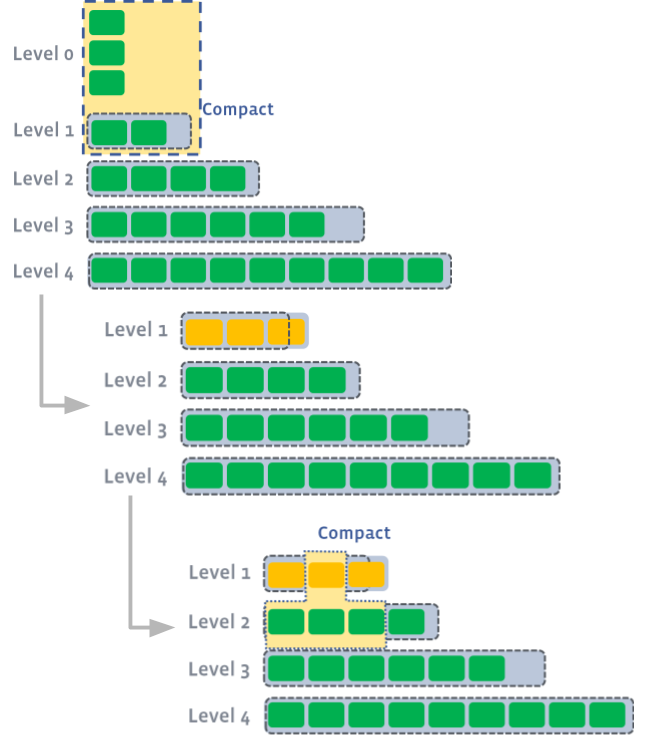
\includegraphics[width=0.5\textwidth]{level_compaction}
  \caption{SS-tables from initial levels are compacted into the next~\cite{rocksdb-compaction}.}
\end{figure}

In RocksDB, compactions are triggered when the previous \textit{level} reaches a
certain size. Referred to as \textit{leveled compaction}, this was one of the
original contributions of LevelDB\@. As described in~\cite{rocksdb-compaction},
compactions are usually initiated when the SS-table count at the first level,
level 0, goes beyond a certain amount. This in turn might cause the next level
to go beyond its size limit, resulting in a compaction to the next level again,
and so on. Unlike LevelDB, RocksDB also supports doing compactions in parallel,
as long as there are enough available background threads to do so.

\subsection{Bloom filters}\label{sec:bloom}

Iterating through every SS-table available to find a single key is inefficient.
Instead, we would like to ask the question ``can this key possibly exist here?''
for each of the SS-tables we go through, and only operate on the ones where the
answer is affirmative. With a regular hash based data structure this would be
quite costly in terms of space, as we would need to maintain such a structure
for every SS-table in our database. Instead, RocksDB, and many other systems
like it, rely on a probabilistic data structure known as a bloom
filter~\cite{bloom} to do so.

Instead of knowing with 100\% certainty whether a key exists in a set, a bloom
filter would let us know if that key \textit{might possibly} be in the set, or
if it is \textit{definitely} not. The third option, of \textit{possibly not}
being in the set, is impossible. The positive trade-off here is that it uses
significantly less space, allowing it to be used for every SS-table in the
system.

\subsection{Iteration}
One of the essential features of RocksDB compared to other key-value stores is
that its data is \textit{sorted}, and that it can be queried as such through
\textit{iterators}. This opens for a wide variety of possibilities that would
not have been feasible with a regular key-value store, such as range queries.
RocksDB supports iterating both forwards and backwards.

Similar to with reads, performing a fully ordered scan in an LSM-tree based
storage engine is far from optimal: every tree-structure, or SS-table in
RocksDB, needs to be considered, and as key ranges may overlap between different
files, sorted.

A lot of applications do not rely on completely random scans of keys however,
and only need support for ordered queries within a specific \textit{key prefix}.
Developers instruct RocksDB on how to retrieve a specific prefix from each key,
which RocksDB then internally uses to organize the data in such a manner that
iterating through keys within a \textit{specific prefix} is efficient: either by
storing bloom filters for each prefix, or by managing a hash based index
structure based on the prefix.

% TODO: might show an example to better explain prefix stuff here, or save it
% for implementation.

\subsection{Column Families}

RocksDB supports the equivalent of tables from a traditional database through
\textit{column
families}\furl{https://github.com/facebook/rocksdb/wiki/Column-Families}.
Separate column families share the same write-ahead log but have their own
MemTables and SS-tables. Maintaining the same WAL makes it possible to
atomically write across multiple column families, while keeping independent
LSM-tree components open for the possibility of configuring different column
families separately---an important difference from tables in SQL databases.

Column family support was not added until version 3.0 of RocksDB.\@ To maintain
backwards compatibility, the default API methods operate on the same column
family, ``default'', with separate methods taking in an additional column family
argument.

\subsection{Customizing the MemTable implementation}\label{sec:memtable-impl}

RocksDB provides multiple implementations of its in-memory
MemTable\furl{https://github.com/facebook/rocksdb/wiki/MemTable}, which can be
changed between through \textit{factories}. Different implementations have
different advantages and disadvantages, with the default being the all around
safest choice.

\subsubsection{Skip list}

The default implementation uses a \textit{skip list}, a data structure with
comparable performance guarantees to a binary search tree---$ O(\log n) $ for
searches, insertions and deletions---but with far better support for concurrent
operations. This makes the default skip list implementation the only MemTable
factory capable of concurrent insertions. Flushing a skip list MemTable to disk
is also considerably faster compared to the other factories, with a much lower
memory overhead.

\subsubsection{Hash skip list}

RocksDB provides two hash based MemTable factories, where keys are organized in
buckets based on their extracted \textit{prefix}. This implies that the hash
based implementations are only usable when a prefix extractor is defined, and
that they only support efficient iterations within a specific prefix. At the
same time, the hash based implementations are also considerably more efficient
when that is the case, providing $ O(\log k) $ performance, where $ k $ is the
number of keys within a specific prefix (which is often quite low).

\subsubsection{Hash linked list}

Similar to the skip list based hash table, RocksDB also provides a hash based
implementation where each bucket is maintained as a linked list instead of a
skip list. This is similar to a traditional hash table with chaining as its
collision resolution, and maintains close to constant time performance
guarantees as long as the elements in each bucket is kept low. This comes with
significantly lower memory overhead compared to the skip list based hash table,
but with naturally lower performance when the amount of keys per prefix starts
to grow. Because of this, the buckets in a \code{HashLinkList} are implicitly
converted to a skip list when its element count exceeds a certain threshold (256
by default).

\subsubsection{Vector}

Finally, RocksDB also provides a MemTable factory heavily tuned for random
insertions, with abysmal performance for everything else. This makes it only
useful for bulk loading data as fast as possible.

\subsection{Customizing the SS-table implementation}\label{sec:ss-table}

The default SS-table implementation is based on the original format from
LevelDB,
\code{BlockBasedTable}\furl{https://github.com/facebook/rocksdb/wiki/Rocksdb-BlockBasedTable-Format}.
As the name implies, data is stored in separate blocks, where each file's
initial block is a filter on the rest of the contents. The size of a single
block is usually fixed and can be configured by the application. Read operations
always read an entire block into memory, before searching for a specific record.
Previously read blocks are maintained in an in-memory cache---a block cache.

RocksDB also provides an improved format designed for low query latency on
modern storage media,
\code{PlainTable}\furl{https://github.com/facebook/rocksdb/wiki/PlainTable-Format}.
The format was initially developed for in-memory databases, but performs well on
other high performance mediums as well. Unlike \code{BlockBasedTable},
\code{PlainTable} addresses records by row, and uses a hash based in-memory
index for efficient reads. Similar to the hash based MemTable formats described
in section~\ref{sec:memtable-impl}, it uses \textit{prefix extraction} to place
keys into separate buckets. This also limits seek-based iteration to a single
prefix.

\subsection{RocksDB from Rust}\label{sec:rust-rocksdb}
While RocksDB is written in C++, it provides a separate API through its
C-bindings, which are used to call into it from a variety of different
languages\furl{https://github.com/facebook/rocksdb/blob/master/LANGUAGE-BINDINGS.md}.

% TODO: ref to appendix?
% TODO: ref to ffi section
This thesis makes use of a modified version of
\code{rust-rocksdb}\furl{https://github.com/spacejam/rust-rocksdb}, which
exposes a Rust-friendly API that calls into the C-bindings. The
majority of the modifications are listed in appendix A.

\begin{listing}[H]
  \begin{minted}[frame=lines]{rust}
let db = DB::open_default("db_path").unwrap();

let key = b"key";
let value = b"value";
db.put(key, value).unwrap();

match db.get(key) {
  Ok(v) => assert_eq!(*v.unwrap(), value),
  Err(e) => panic!("failed reading from rocksdb: {}", e),
}
  \end{minted}

  \caption{Simple example usage of rust-rocksdb}\label{lst:rocksdb-rust}
\end{listing}

\section{Rust}\label{sec:rust}

Rust\furl{https://www.rust-lang.org/} is an open-source systems programming
language spearheaded by Mozilla, where it is used to build Servo---a next
generation browser engine\furl{https://servo.org/}. Rust provides memory safety
without the runtime overhead of \eg garbage collection, making it a suitable
language for everything from embedded systems to web service backends.

When choosing a programming language, developers are often forced to compromise
between higher level abstractions and performance. Large and latency sensitivity
projects like databases often opt for the latter through low-level languages
like C, which avoid expensive runtime safety checks. Rust removes this dilemma
altogether by providing developers with both the fine-tuned control and
performance they are used to in low-level languages, while offering abstractions
developers might be familiar with from interpreted languages.

% TODO: avoid expensive runtime safety checks is a weird sentence

\begin{listing}[H]
  \begin{minted}[frame=lines]{rust}
fn suffix(input: &mut String) {
    input.push_str(" is a String!");
}

fn output(input: String) {
    println!("Hello: {}", input);
}

fn main() {
    // Construct a mutable String, from a string litteral (str):
    let mut input = String::from("Hi!");
    // Pass a mutable reference to suffix:
    suffix(&mut input);
    // Finally, move our input variable into the output function:
    output(input);
    // println!("This line would not compile: {}", input);
}
  \end{minted}
  \caption{\
    The example shows the basics of Rust's move semantics. The \texttt{input}
    variable cannot be used after the call to \texttt{output()}, as it has been
    \textit{moved} into the function.
  }
\end{listing}

One of Rust’s key features is providing compile time safety both in terms of
types and memory. The latter is done through an ownership model which lets
developers program mostly without thinking about memory allocation and
deallocation, without the lowered performance of using something like a garbage
collector. Each variable in Rust is assigned one and only one owner, and the
variable is deallocated when that owner goes out of scope.

% TODO: write a little more here

\subsection{Foreign Function Interface}\label{sec:ffi}

Rust has excellent support for calling into C programs, which lets developers
access the myriad of libraries written in C, together with C++ programs that
provide C interfaces. To call external programs, developers define each external
function in a \textit{foreign function
interface}\furl{https://doc.rust-lang.org/book/first-edition/ffi.html}, through
use of the \code{extern} keyword, which also supports linking to external
libraries.

\begin{listing}[H]
  \begin{minted}[frame=lines]{rust}
extern "C" {
  fn rand() -> i32;
}

fn main() {
  unsafe {
    println!("Random number: {}", rand());
  }
}
  \end{minted}
  \caption{\
    By defining \code{rand} from the C standard library as an external function,
    we can call it from our Rust program.
  }\label{lst:extern}
\end{listing}

Note that the call to \code{rand} in listing~\ref{lst:extern} needs
to be wrapped in an \code{unsafe} block. While Rust can ensure the safety of
\textit{Rust} code at compile time, it cannot not do so for third-party
applications written in other languages. By introducing the \code{unsafe}
keyword, the blocks of code the developer is forced to maintain the safety of is
isolated to the smallest possible region.

In the same manner, Rust supports defining an interface that can be called from
other languages, such as C, as shown in listing~\ref{lst:call-extern}. This is
especially useful for libraries that require functions as arguments, \eg callbacks.

\begin{listing}[H]
  \begin{minted}[frame=lines]{rust}
#[no_mangle]
pub extern "C" fn multiply(a: i32, b: i32) -> i32 {
  a * b
}
  \end{minted}
  \caption{\
    The \code{multiply} functions can be called through the C-calling convention
    by other programs. The \code{no\_mangle} pragma ensures the \code{multiply}
    name stays unmodified by the compiler.
  }\label{lst:call-extern}
\end{listing}

\section{\code{bincode}}\label{sec:bincode}

\code{bincode}~\cite{bincode} is a binary serialization library, used heavily
throughout both this thesis and in Soup, for everything from RPC
communication to persisting data to durable storage. In short, \code{bincode} takes an
arbitrary Rust object and turns it into a series of bytes---an encoded object.
The size of the resulting byte stream is usually either less than, or the same
as, the size of the source object. \code{bincode} builds on top of the
\code{Serde}\furl{https://serde.rs/} serialization framework.

As the encoded format is of relevance to later sections, we will briefly go
through it here. Primitive values, such as numbers, are encoded directly using
Rust's \code{Writer} trait, with a few exceptions:

\begin{itemize}
  \item \code{isize} and \code{usize} types, which have varying sizes depending
    on the OS, are encoded as \code{i32} and \code{u64} correspondingly.
  \item Strings are encoded as the tuple \code{(number of bytes, bytes)}, where
    the former is a \code{u64} and the latter is a byte slice.
\end{itemize}

Compound types---enums, structs, vectors, and tuples---are encoded recursively,
with each of their fields placed out in succession. With vector lengths not
being determined at compile time, vectors are prefixed with a length field on
the form of a \code{u64}. This is not necessary for the other compound types, as
their sizes do not vary at runtime. An enum instance can represent multiple
types, and is prefixed with a \code{u32} tag used to determine which
enum variant it represents.

\begin{listing}[H]
  \begin{minted}[frame=lines]{rust}
#[derive(Serialize, Deserialize, Debug, PartialEq)]
enum Number {
    Positive(u64),
    Negative(u64)
}

fn main() {
    let values = vec![Number::Positive(3), Number::Negative(4)];
    // This serializes as:
    // vector length u64,
    // + enum variant u32 + u64,
    // + enum variant u32 + u64
    // = u64, u32, u64, u32, u64
    // = 32 bytes
    let raw = bincode::serialize(&values).unwrap();
    let deserialized: Vec<_> = bincode::deserialize(&raw).unwrap();

    for (i, element) in values.into_iter().enumerate() {
        assert_eq!(element, deserialized[i]);
    }
}
  \end{minted}

  \caption{\
    Types implementing the \code{Serialize} and \code{Deserialize} traits can be
    encoded and decoded using \code{bincode}.
  }\label{lst:bincode}
\end{listing}


\section{Profiling}

\subsection{CPU}

A large part of application performance tuning comes down to figuring out which
portion of a program is running slowly and why that is the case. Throughout
this thesis that is accomplished using
\code{perf}\furl{https://perf.wiki.kernel.org}---a profiling tool that helps us
answer the question ``What is the CPU spending time on?''.

\code{perf} collects information from both hardware counters and logical
tracepoints. The latter is especially useful for recording call graphs of a
program, which in turn lets us produce flame graphs like the one in
figure~\ref{fig:flame-example}, using tools such as
\code{FlameGraph}\furl{https://github.com/brendangregg/FlameGraph} and
\code{FlameScope}\furl{https://github.com/Netflix/flamescope}. Flame graphs show
time spent on the horizontal axis, while showing the call graph vertically.

\begin{figure}[H]
  \centering
  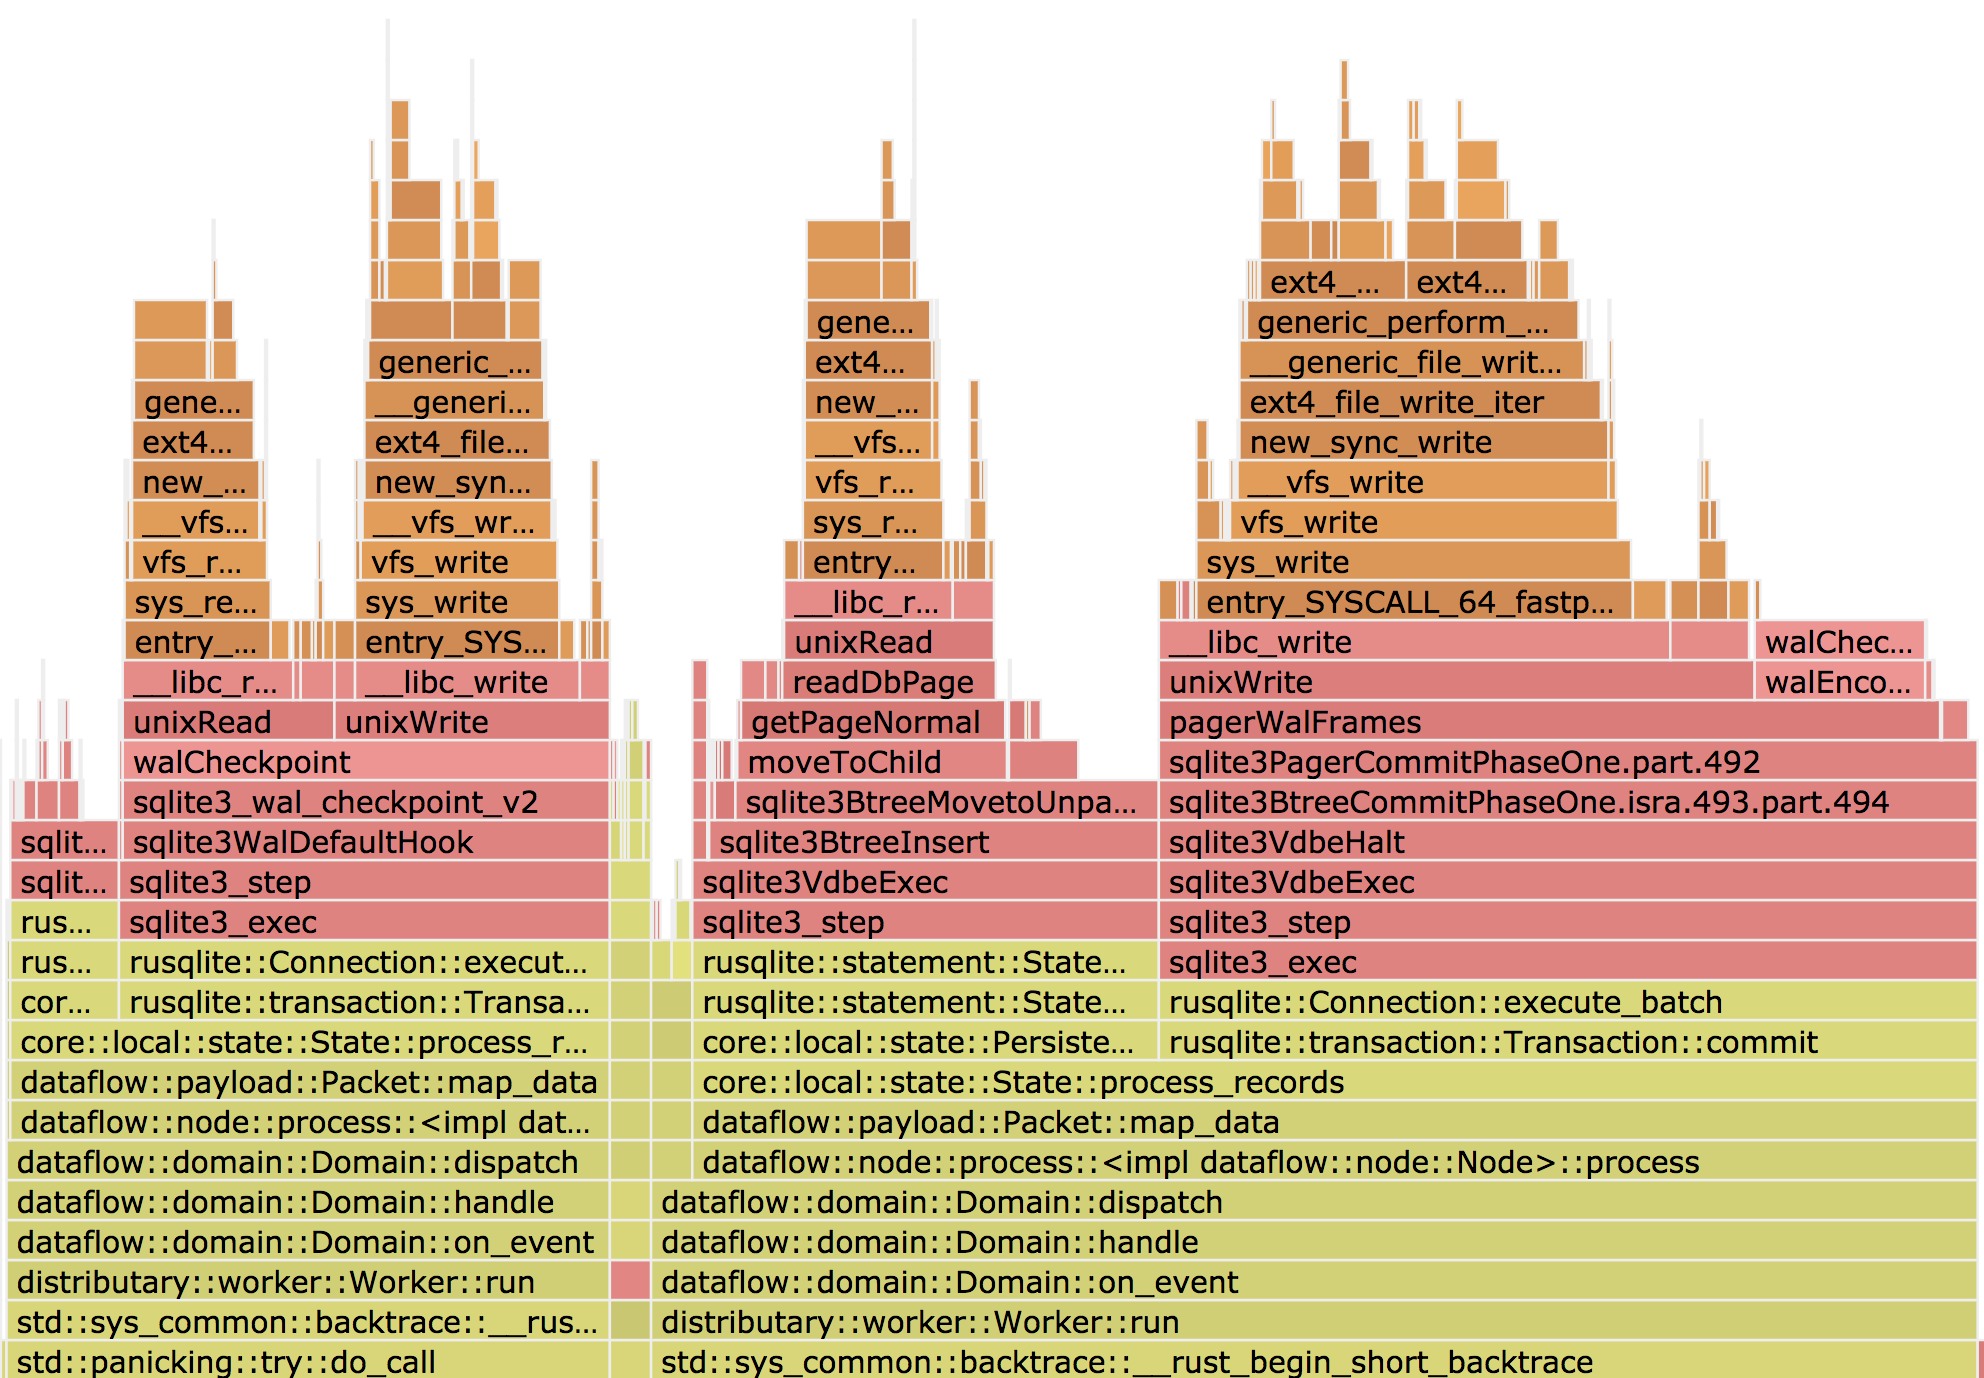
\includegraphics[width=\textwidth]{flame-example}
  \caption{\
    An example flame graph from events recorded using \code{perf}.
  }\label{fig:flame-example}
\end{figure}

\subsection{Memory}

% TODO: shitty sentence
Memory leaks happen when we continually allocate memory without freeing it. This
can easily happen in languages without dynamic memory allocation, when a
programmer forgets to deallocate some portion of memory after using it. At the
same time it can also happen in garbage collected languages, \eg when
continuously attaching listener functions to an event system without regard for
previous subscriptions. Rust's ownership system largely prevents issues of the
first kind from happening---variables that go out of scope are deallocated
automatically. Regardless, Rust supports calling into arbitrary C-programs (see
section~\ref{sec:ffi}), where anything could happen.

To profile memory leaks, the Valgrind
Massif\furl{http://valgrind.org/docs/manual/ms-manual.html} heap profiler is
used. Massif continuously takes snapshots of the heap, recording what memory is
used for, and where that memory was allocated from. While this is subject to
change in the future, current versions of Rust use the
\code{jemalloc}\furl{http://jemalloc.net/} memory allocator instead of the
system's default allocator. Unfortunately, memory profiling using Valgrind does
not work well with \code{jemalloc}. To resolve this we can instead force Rust to
use the system allocator, at least while profiling.

\begin{listing}[H]
  \begin{minted}[frame=lines]{rust}
#![feature(alloc_system)]
#![feature(global_allocator, allocator_api)]

#[global_allocator]
static ALLOC: std::alloc::System = std::alloc::System;
  \end{minted}

  \caption{Forcing Rust to use the system memory allocator makes it possible to
  profile it using tools such as Valgrind Massif.}\label{lst:system-alloc}
\end{listing}

